% !TEX TS-program = xelatex
% !BIB TS-program = bibtex
\documentclass[12pt,letterpaper]{article}
\usepackage{style/dsc180reportstyle} % import dsc180reportstyle.sty
\usepackage{float} % for [H] figure placement

%%%%%%%%%%%%%%%%%%%%%%%%%%%%%%%%%%%%%%%%%%%%%%%%%%%%%%%%
%%%% Title and Authors
%%%%%%%%%%%%%%%%%%%%%%%%%%%%%%%%%%%%%%%%%%%%%%%%%%%%%%%%

\title{DSC Capstone Q2 Report}

\author{Jevan Chahal\\
  {\tt j2chahal@ucsd.edu} \\\And
  Hillary Change \\
  {\tt hic001@ucsd.edu} \\\And
  Kurumi Kaneko \\
  {\tt kskaneko@ucsd.edu} \\\And
  Kevin Wong \\
  {\tt kew024@ucsd.edu} \\\And
  Brian Duke \\
  {\tt brian.duke@prismdata.com} \\\And
  Kyle Nero \\
  {\tt kyle.nero@prismdata.com} \\}

\begin{document}
\maketitle

%%%%%%%%%%%%%%%%%%%%%%%%%%%%%%%%%%%%%%%%%%%%%%%%%%%%%%%%
%%%% Abstract and Links
%%%%%%%%%%%%%%%%%%%%%%%%%%%%%%%%%%%%%%%%%%%%%%%%%%%%%%%%

\begin{abstract}
    \textcolor{black}{
    The process of capturing what makes a creditor trustworthy or not is especially vital within the confines of bank data, due to the guidelines and ethics of what makes this data usable. Although the quantity of the data is massive, there are only a few available features that are explicitly useful in the confines of machine learning, which calls into question how we should measure customer's trustworthiness towards their creditors. Our methodology details the process of refining bank data into categories using Natural Language Processing, assessing individual's income based on bank data alone, and also measuring their credit worthiness both accurately and efficiently. 
    }
\end{abstract}

\begin{center}
Code: \url{https://github.com/hillarychang/dsc180b-capstone-q2}
\end{center}

\maketoc
\clearpage

%%%%%%%%%%%%%%%%%%%%%%%%%%%%%%%%%%%%%%%%%%%%%%%%%%%%%%%%
%%%% Main Contents
%%%%%%%%%%%%%%%%%%%%%%%%%%%%%%%%%%%%%%%%%%%%%%%%%%%%%%%%
\section{Introduction}

Access to credit is crucial for financial stability, yet traditional credit scoring models often exclude individuals with limited credit history. The "Cash Score" project aims to address this issue by utilizing transaction data to evaluate financial behaviors rather than just historical credit data. Our goal is to provide a more equitable scoring system that benefits both consumers and financial institutions.

\subsection{Data Description}
We utilized multiple datasets that provide consumer transaction details, account balances, and delinquency indicators:
\begin{itemize}
    \item \textbf{q2-ucsd-consDF.pqt}: Contains consumer attributes like \texttt{consumer\_id}, \texttt{credit\_score}, and \texttt{DQ\_target} (delinquency indicator).
    \item \textbf{q2-ucsd-acctDF.pqt}: Includes account-level data such as \texttt{consumer\_id}, \texttt{account\_id}, \texttt{balance\_date}, and \texttt{balance}.
    \item \textbf{q2-ucsd-trxnDF.pqt}: Captures transactional details including \texttt{category}, \texttt{amount}, \texttt{credit\_or\_debit}, and \texttt{posted\_date}.
    \item \textbf{categories.csv}: Maps transaction categories like Rent, Groceries, and Entertainment.
\end{itemize}

\begin{figure}[H]
    \centering
    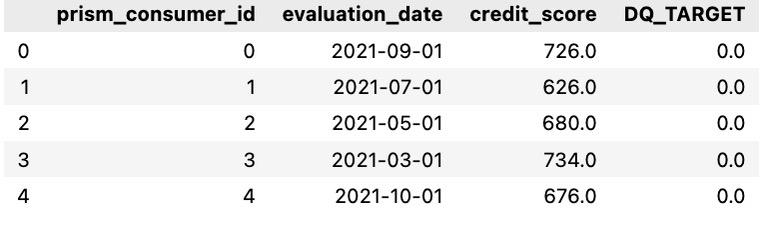
\includegraphics[width=\textwidth]{figure/consumer_df.jpeg}
    \caption{First few columns of the consumer dataset, including consumer ID, evaluation date, credit score, and delinquency target.}
    \label{fig:consumer_df}
\end{figure}

\begin{figure}[H]
    \centering
    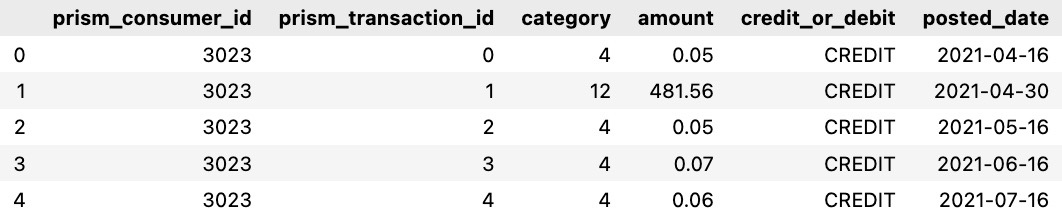
\includegraphics[width=\textwidth]{figure/transactions_df.jpeg}
    \caption{First few columns of the transactions dataset, showing transaction IDs, categories, amounts, and whether they were credit or debit.}
    \label{fig:transactions_df}
\end{figure}

\begin{figure}[H]
    \centering
    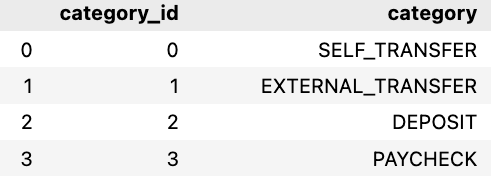
\includegraphics[width=0.7\textwidth]{figure/categories_df.png}
    \caption{First few columns of the transaction categories dataset, mapping category IDs to their corresponding descriptions.}
    \label{fig:categories_df}
\end{figure}


\begin{figure}[H]
    \centering
    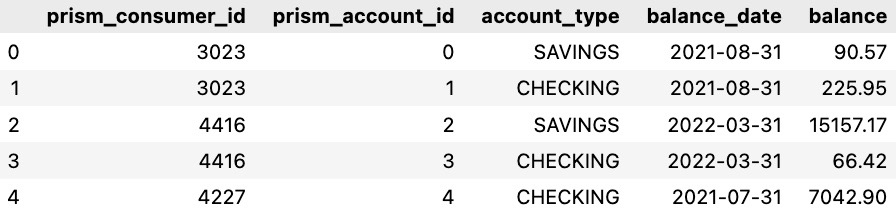
\includegraphics[width=\textwidth]{figure/accounts_df.jpeg}
    \caption{First few columns of the accounts dataset, including account IDs, account types, balance dates, and balances.}
    \label{fig:accounts_df}
\end{figure}

\begin{figure}[H]
    \centering
    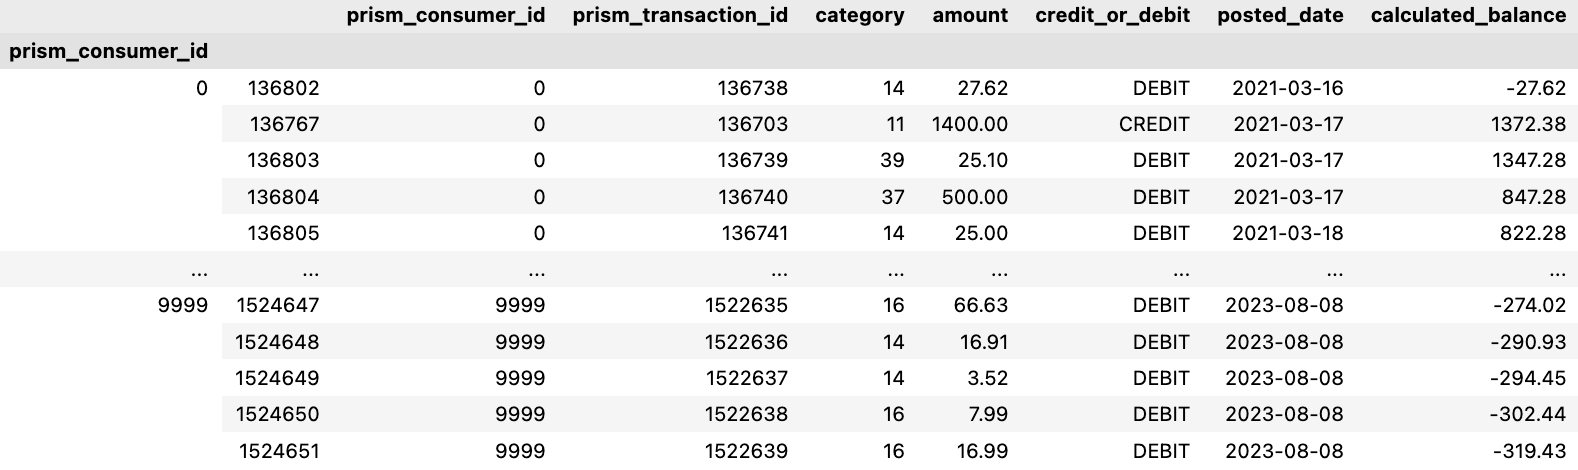
\includegraphics[width=\textwidth]{figure/final_transaction_balance.png}
    \caption{Dataframe showing all user transactions along with their account balances. Credit transactions (inflows) are added while debit transactions (outflows) are subtracted.}
    \label{fig:final_transaction_balance}
\end{figure}


\section{Methodology}

\subsection{Exploratory Data Analysis}
\begin{itemize}
    \item Identified differences in transaction patterns between delinquent and non-delinquent consumers.
    \item Examined seasonal trends, payday effects, and spending fluctuations.
    \item Estimated income using reoccuring transactions
    \item Analyzed the impact of account fees, buy-now-pay-later (BNPL) transactions, and overdrafts.
\end{itemize}

\subsection{Balance Trends for Delinquent vs. Non-Delinquent Consumers}

\begin{figure}[H]
    \centering
    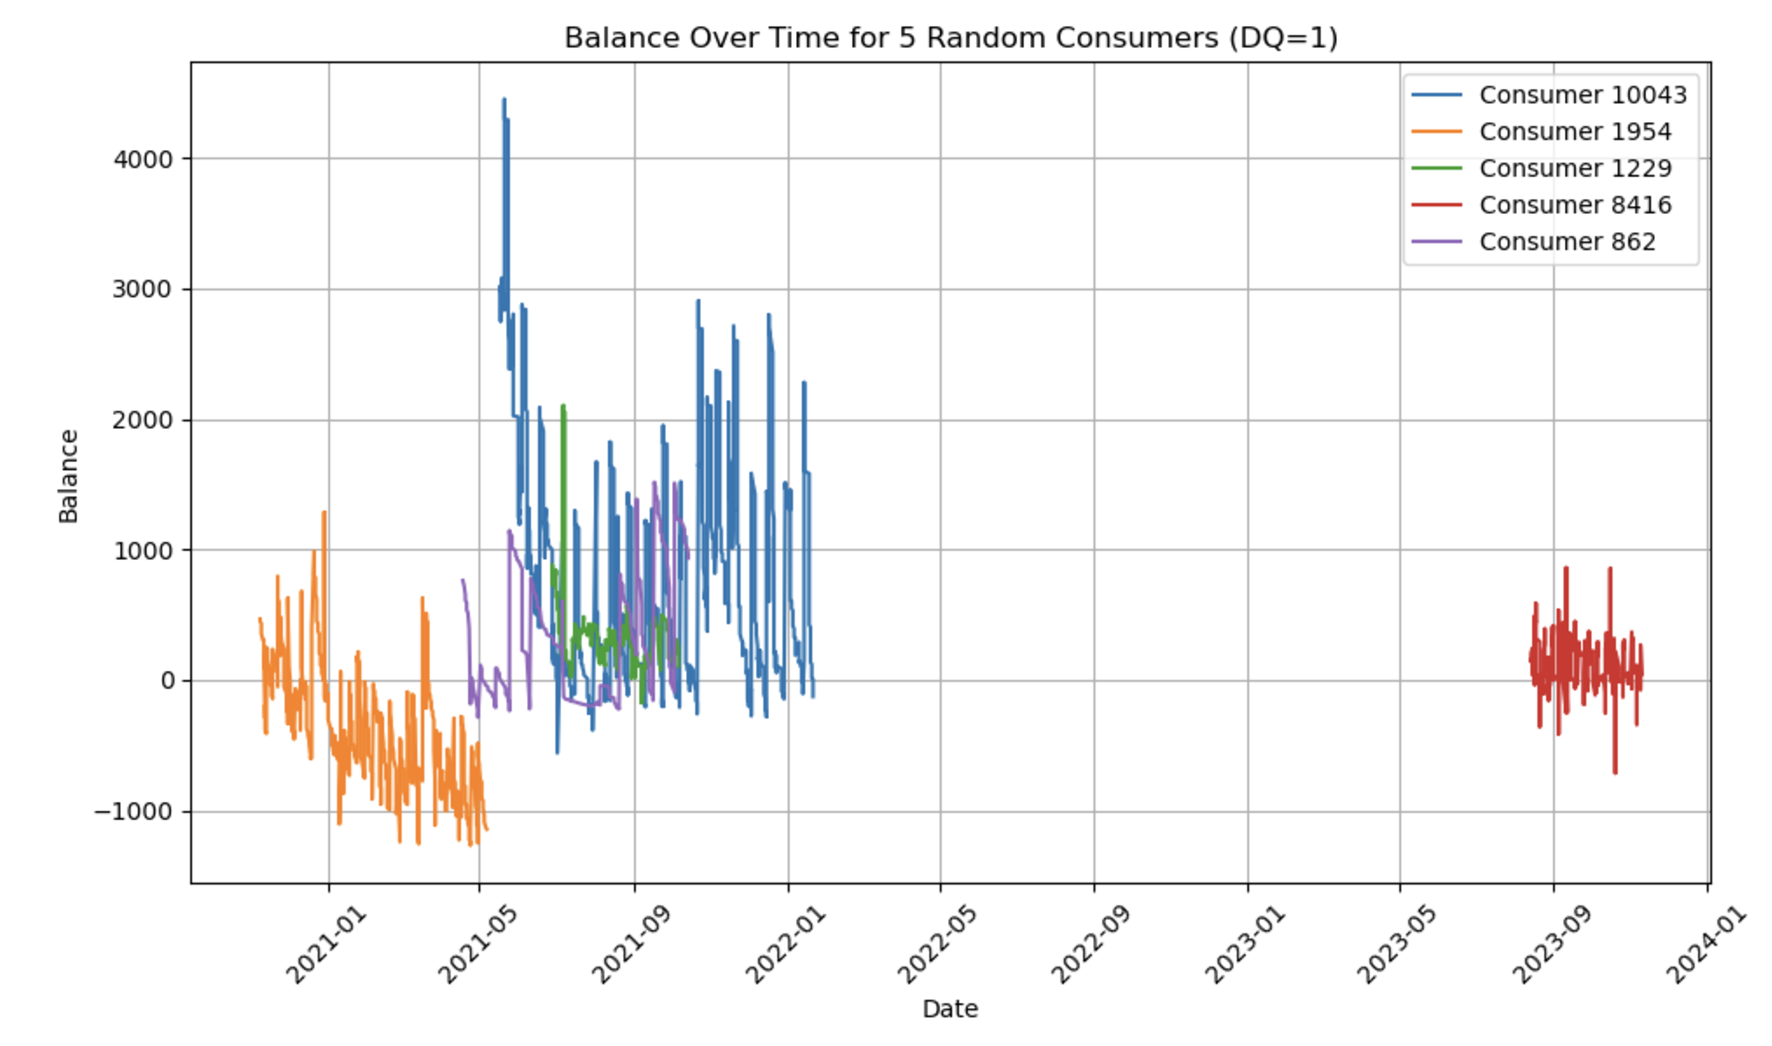
\includegraphics[width=0.7\textwidth]{figure/balance_delinquent.png}
    \caption{Balance trends over time for five randomly selected delinquent consumers. The plot illustrates fluctuations and frequent occurrences of negative balances, highlighting financial instability.}
    \label{fig:balance_delinquent}
\end{figure}

\begin{figure}[H]
    \centering
    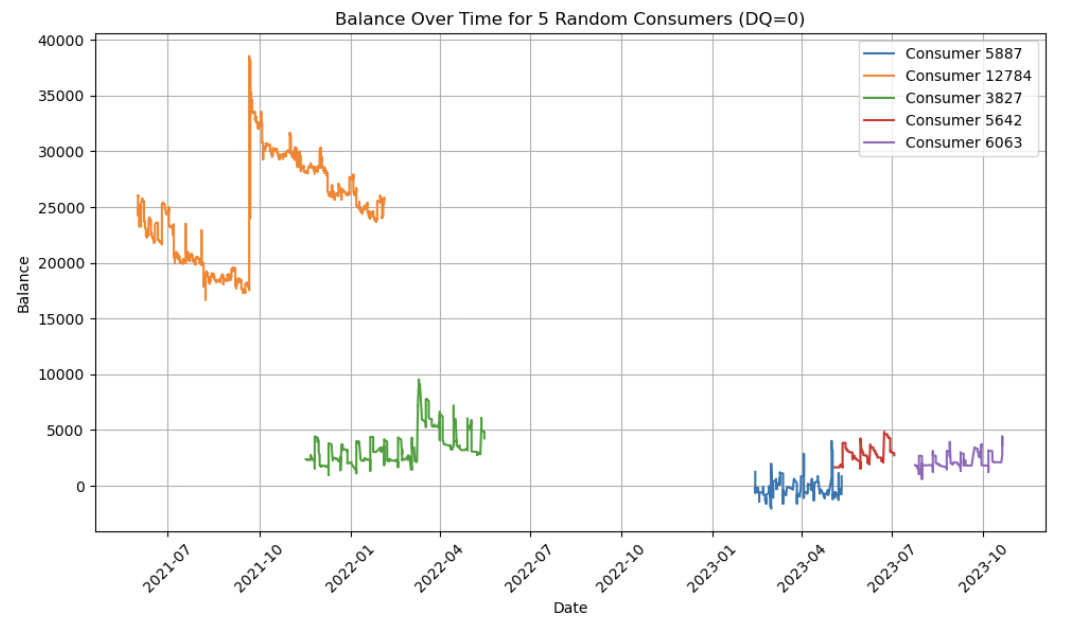
\includegraphics[width=0.7\textwidth]{figure/balance_non_delinquent.png}
    \caption{Balance trends over time for five randomly selected non-delinquent consumers. Compared to delinquent consumers, these users maintain more stable balances with fewer instances of overdrafts.}
    \label{fig:balance_non_delinquent}
\end{figure}

\begin{figure}[H]
    \centering
    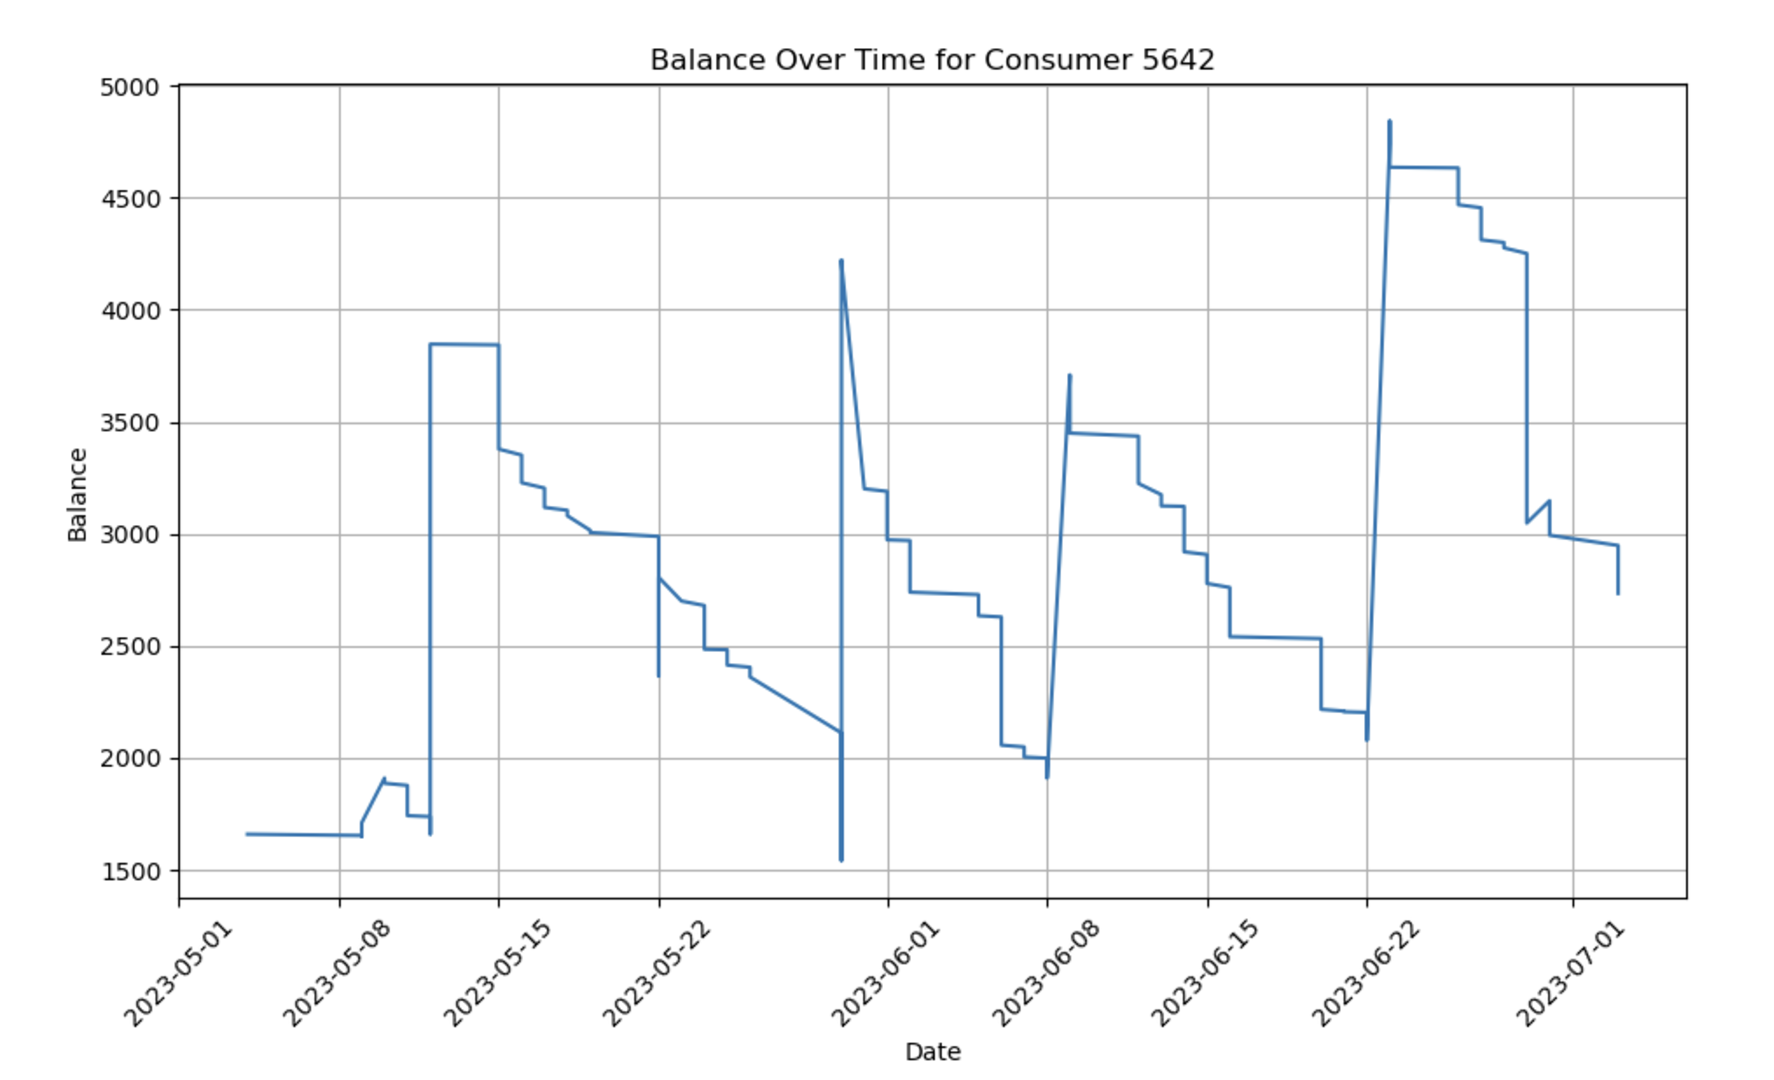
\includegraphics[width=0.7\textwidth]{figure/balance_single_non_delinquent.png}
    \caption{Balance over time for a single non-delinquent consumer. The balance exhibits periodic fluctuations, potentially due to income deposits and spending patterns, but remains above zero during the observed period.}
    \label{fig:balance_single_non_delinquent}
\end{figure}

\begin{figure}[H]
    \centering
    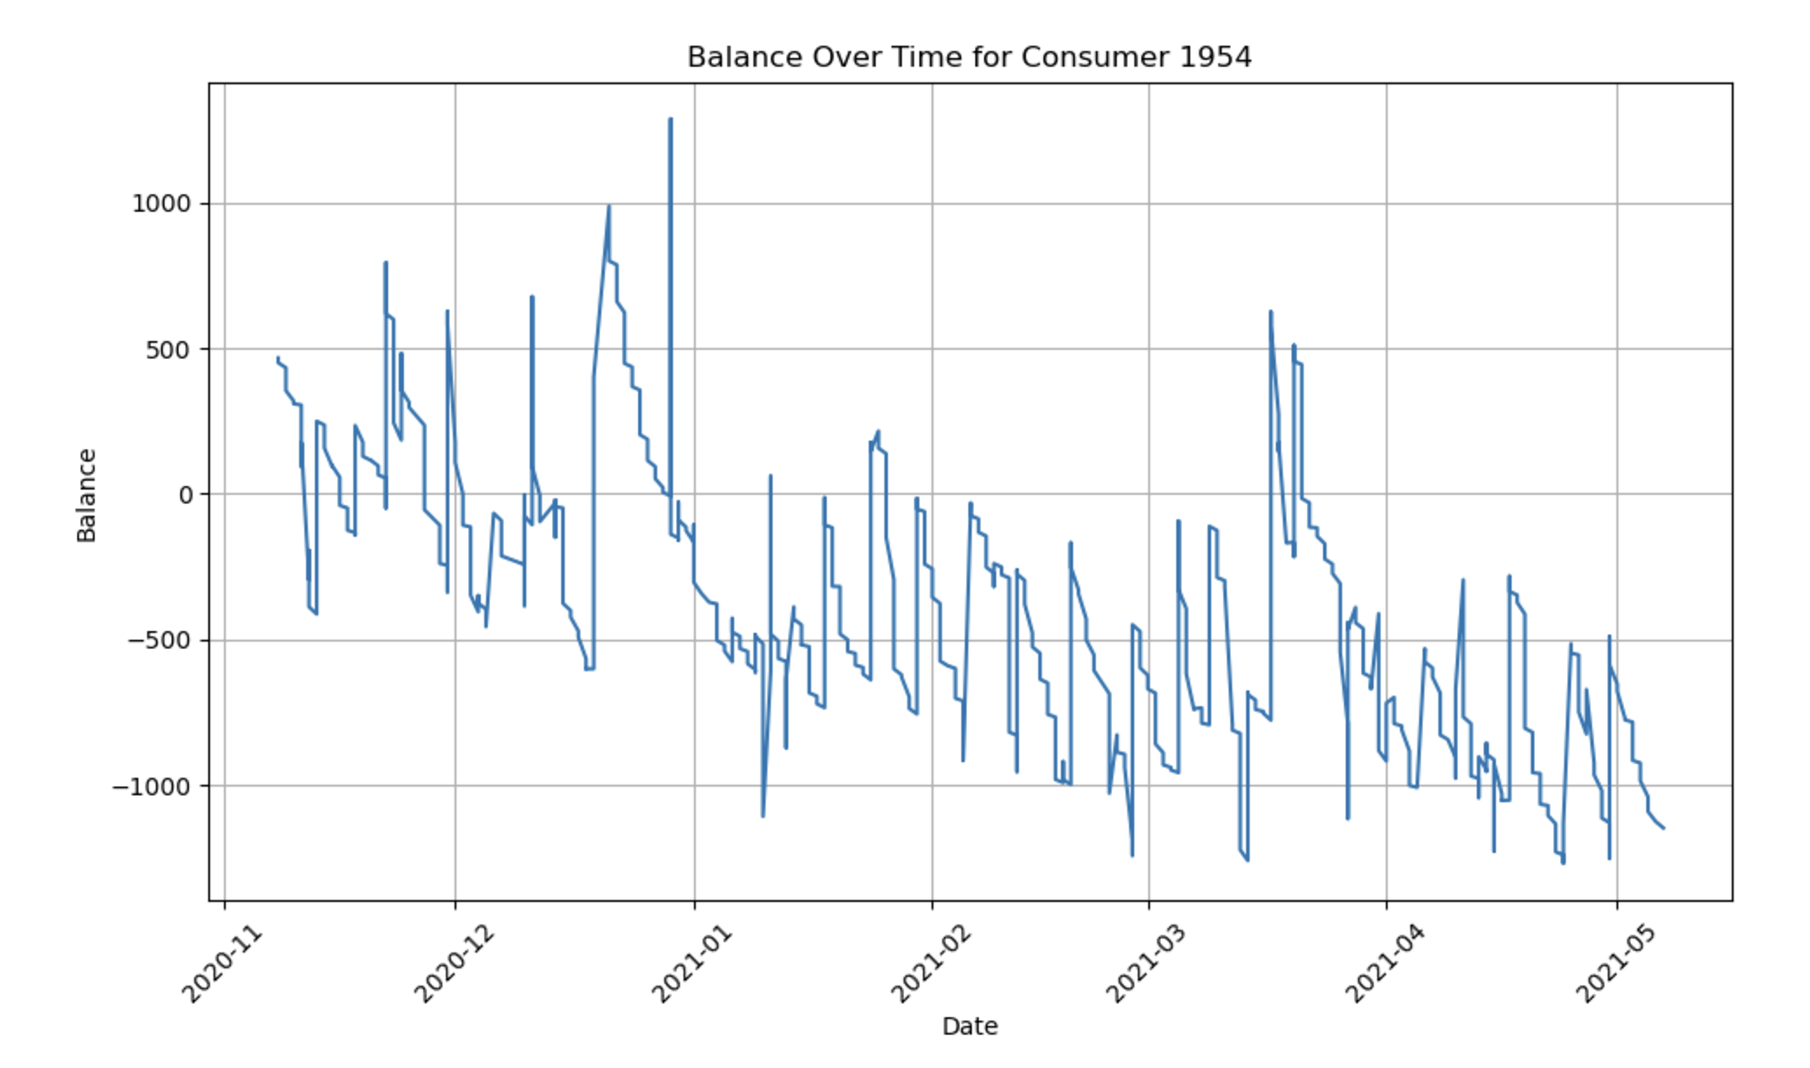
\includegraphics[width=0.7\textwidth]{figure/balance_single_delinquent.png}
    \caption{Balance over time for a single delinquent consumer. This consumer frequently experiences negative balances, indicating financial distress and an increased risk of missing payments.}
    \label{fig:balance_single_delinquent}
\end{figure}


\subsection{Feature Engineering}
We engineered multiple features relevant to the prediction of delinquency:
\begin{itemize}
    \item \textbf{Balance Features}: Negative balance ratio, balance trends, payday effects.
    \item \textbf{Transaction-Based Features}: Credit vs. debit transaction volume, category-based spending breakdown.
    \item \textbf{Temporal Features}: Spending frequency over time, account for longevity effects.
    \item \textbf{Account Types}: Features based on the types of accounts a consumer has
\end{itemize}

\begin{figure}[H]
    \centering
    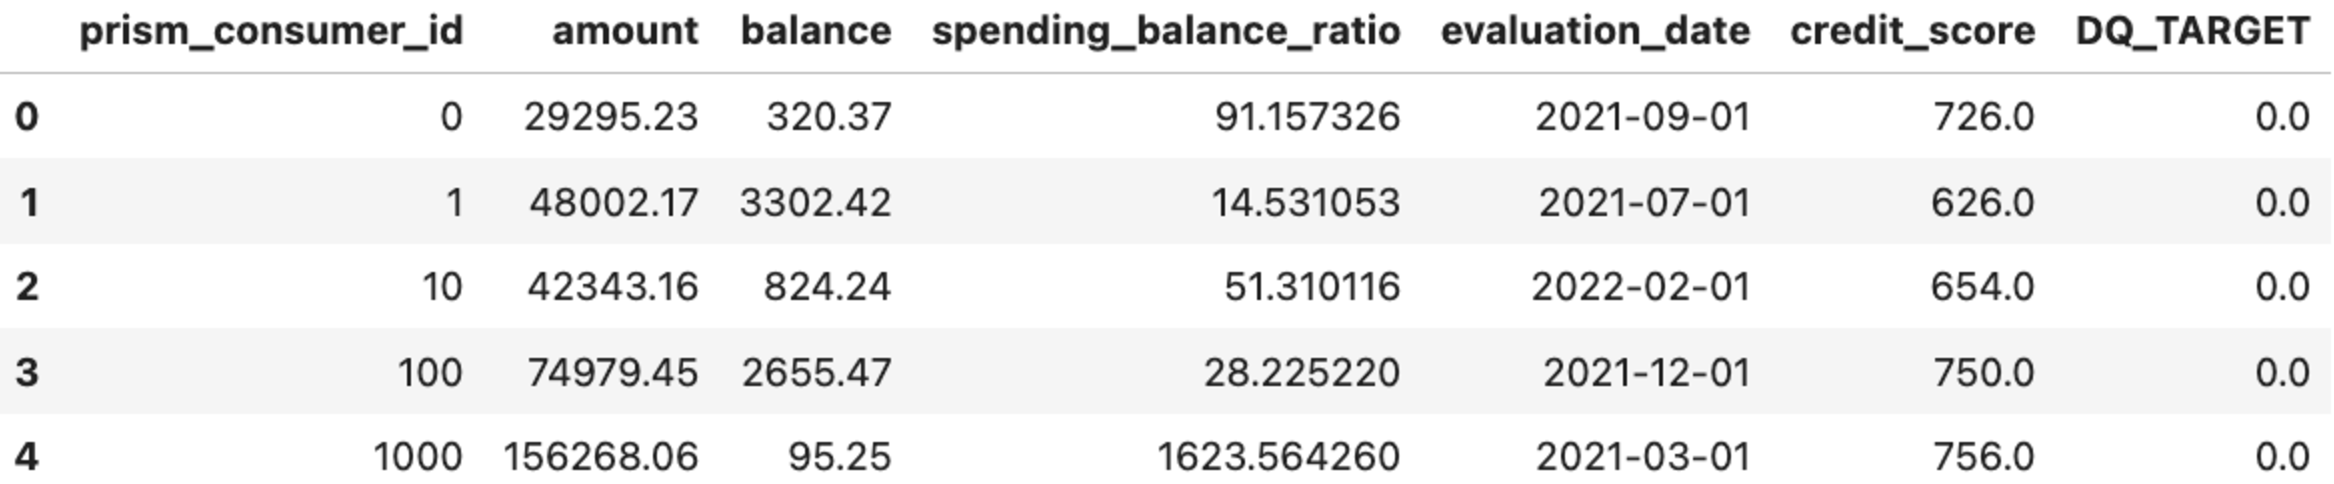
\includegraphics[width=\textwidth]{figure/spending_balance_ratio.png}
    \caption{Spending balance ratio feature created to measure how much consumers spend relative to their balance. This helps assess financial stability and risk of delinquency.}
    \label{fig:spending_balance_ratio}
\end{figure}

\begin{figure}[H]
    \centering
    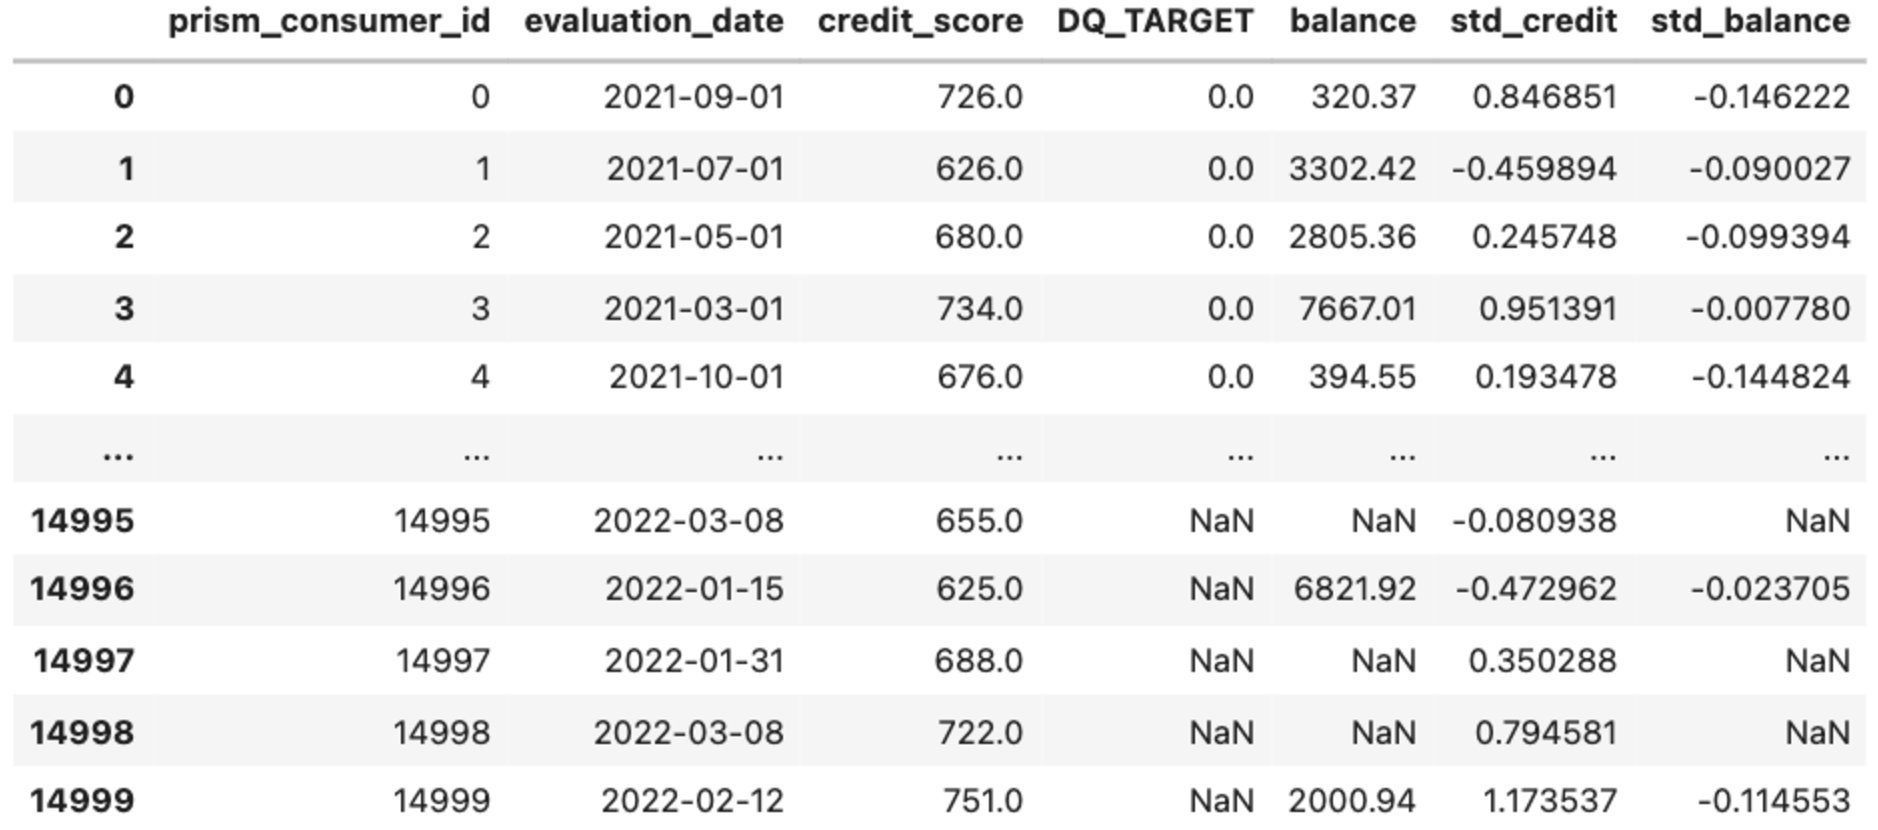
\includegraphics[width=\textwidth]
    {figure/standardized_credit_balance.png}
    \caption{Feature engineering step where credit and balance were standardized to allow for easier model interpretability and comparisons across different financial profiles.}
    \label{fig:standardized_credit_balance}
\end{figure}

\subsection{Model Training}
We trained the following machine learning models:
\begin{itemize}
    \item \textbf{Logistic Regression}: Simple, interpretable baseline model.
    \item \textbf{Random Forest}: Captures non-linear financial relationships.
    \item \textbf{XGBoost}: Optimized for structured financial data.
    \item \textbf{Neural Networks}: Captures complex spending patterns.
    \item \textbf{LightGBM}: Efficient with categorical features and handling imbalanced data.
    \item \textbf{Balanced RF}: Handles class imbalance by weighting classes or resampling.
    \item \textbf{CatBoost}: Handles categorical features automatically, robust to overfitting.
    \item \textbf{HistGB}: A histogram-based gradient boosting model
    \item \textbf{RUSBoost}: Combines Random Under-Sampling with boosting to address class imbalance while maintaining predictive performance.
  
\end{itemize}

\subsection{Model Evaluation}
Key metrics for model evaluation include:
\begin{itemize}
    \item \textbf{Accuracy and F1-Score}: Measures classification performance.
    \item \textbf{ROC-AUC}: Evaluates the model's ability to differentiate delinquent users.
    \item \textbf{Precision and Recall}: Precision measures correct positives; recall measures detected positives.
    \item \textbf{Training Time}: Time required to train the model.
    \item \textbf{Prediction Time}: Time taken to make predictions.
    \item \textbf{Feature Importance}: Highlights predictive variables.
\end{itemize}
To mitigate the class imbalance (delinquents only ~8.4\% of dataset), we used:
\begin{itemize}
    \item \textbf{SMOTE \& SMOTEENN}: Oversampling techniques.
    \item \textbf{Feature Normalization}: Standardization of key variables.
\end{itemize}

\section{Results}

\subsection{Feature Performance}
Key predictors of delinquency (XGBClassifier):
\begin{itemize}
    \item \textbf{Account Type - Savings}: If a consumer has a savings acc
    \item \textbf{Account fees}: Sum of all account fees
    \item \textbf{Credit Score}: Credit score of a consumer
    \item \textbf{Overdraft Median}: Median amount of Overdraft
    \item \textbf{Account fees}: Median amount of Account fees
    \item \textbf{BNPL Std}: Standard Deviation of BNPL transactions
    \item \textbf{Overdraft count}: Number of overdraft transactions
    \item \textbf{Investment Income Median}: Median amount of Investment income
    \item \textbf{Investment Income Count}: Number of Investment income transactions
    \item \textbf{Banking Catch All Std}: Standard deviation of a consumer's transactions within this category
\end{itemize}

\begin{table}[H]
    \centering
    \begin{tabular}{|l|c|c|}
        \hline
        Feature & Importance & Correlation \\
        \hline
        account\_types\_savings & 0.044091 & -0.099071 \\
        account\_fees\_count & 0.037083 & 0.020680 \\
        credit\_score & 0.030284 & -0.249976 \\
        overdraft\_median & 0.026024 & 0.000407 \\
        account\_fees\_median & 0.021387 & 0.001497 \\
        BNPL\_std & 0.021323 & 0.034083 \\
        overdraft\_count & 0.021319 & 0.066101 \\
        investment\_income\_median & 0.018767 & 0.004675 \\
        investment\_income\_count & 0.017630 & -0.026354 \\
        banking\_catch\_all\_std & 0.014733 & -0.010585 \\
        \hline
    \end{tabular}
    \caption{Top Features of XGBClassifier}
    \label{tab:top_features_xgb}
\end{table}

\subsection{Model Performance}
\begin{table}[H]
    \centering
    \begin{tabular}{|l|c|c|c|c|c|c|c|}
        \hline
        Model & ROC-AUC & Accuracy & Precision & Recall & F1-Score \\
        \hline

        HistGB & \textbf{0.842428} & 0.913528 & 0.889776 & 0.913528 & 0.899533 \\
        XGBoost & 0.839279 & 0.910069 & 0.889033 & 0.910069 & 0.898105 \\
        LightGBM & 0.828857 & 0.913912 & 0.889361 & 0.913912 & 0.899373 \\
        CatBoost & 0.823153 & 0.915834 & 0.887905 & 0.915834 & 0.898882 \\
        RUSBoost & 0.805893 & 0.826287 & 0.905010 & 0.826287 & 0.857906 \\
        Random Forest & 0.794283 & 0.915450 & 0.885290 & 0.915450 & 0.897285 \\
        Balanced RF & 0.791598 & \textbf{0.919677} & 0.892594 & \textbf{0.919677} & \textbf{0.902200} \\
        Logistic Regression & 0.761125 & 0.759416 & \textbf{0.906664} & 0.759416 & 0.814041 \\
        \hline
    \end{tabular}
    \caption{Comparison of model performance}
\end{table}

\begin{table}[H]
    \centering
    \begin{tabular}{|l|c|c|}
        \hline
        Model & Training-Time & Prediction-Time\\
        \hline

        HistGB & 8.755626 & TODO \\
        XGBoost & 5.682351 & TODO \\
        LightGBM & 4.397599 & TODO \\
        CatBoost & 42.606373 & TODO \\
        RUSBoost & 23.319771 & TODO \\
        Random Forest & 22.369477 & TODO \\
        Balanced RF & 27.226752 & TODO \\
        Logistic Regression & \textbf{2.352007} & TODO \\
        \hline
    \end{tabular}
    \caption{Comparison of time-based model performance}
\end{table}


\begin{figure}[H]
    \centering
    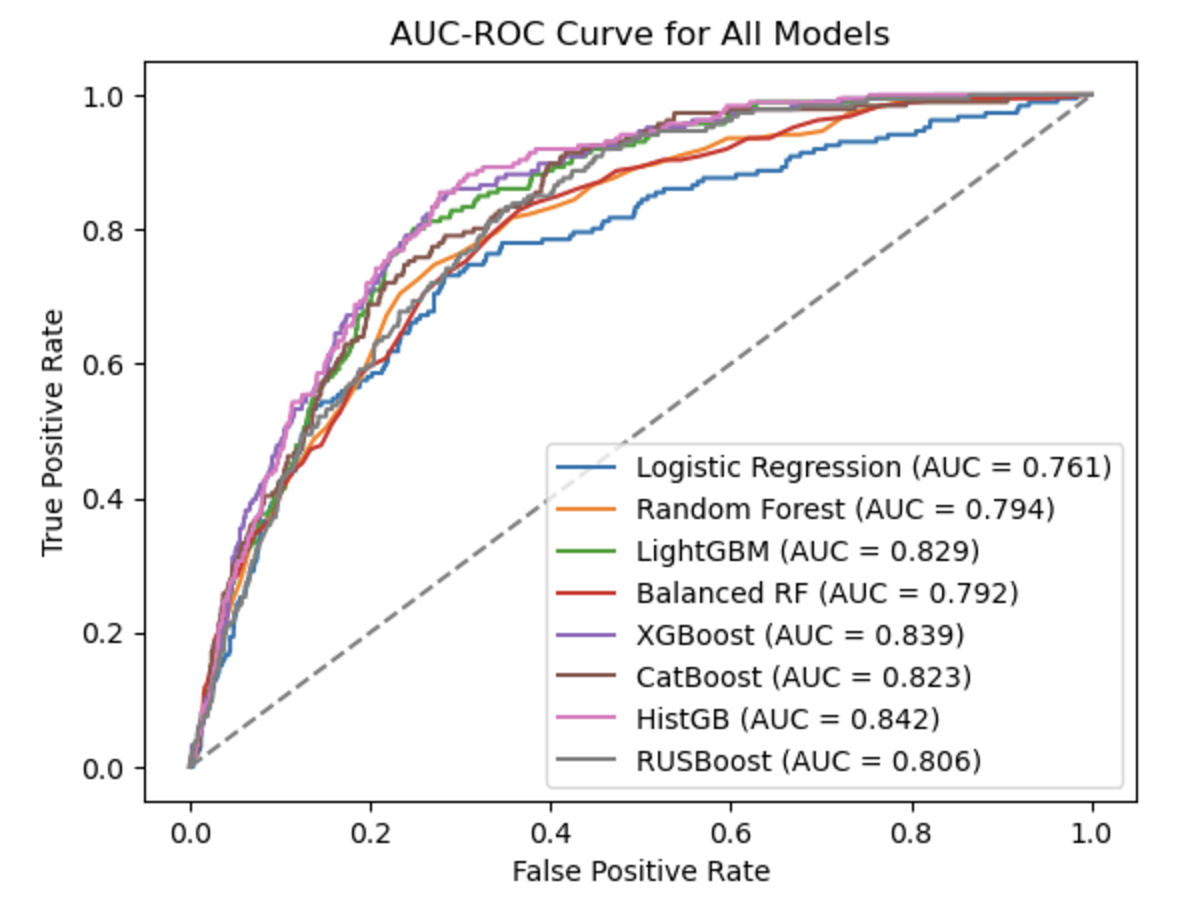
\includegraphics[width=\textwidth]
    {figure/auc_roc_all_models.png}
    \caption{Comparison of all AUC\_ROC scores of the different models we trained.}
    \label{fig:standardized_credit_balance}
\end{figure}

\subsection{Interpretability \& Reason Codes}
Delinquent consumers often had high spending in BNPL and account fees. The top reason codes included:
\begin{itemize}
    \item High balance volatility and overdrafts.
    \item Excessive BNPL spending.
    \item Significant account fees.
\end{itemize}

\section{Conclusion}
We refined predictive features and improved model performance for the assessment of delinquency. By leveraging transaction data, we developed a "Cash Score" that improves upon traditional credit assessments. Future work includes:
\begin{itemize}
    \item Enhancing interpretability with reason codes.
    \item Submitting final model predictions.
    \item Preparing stakeholder presentations.
\end{itemize}

%%%%%%%%%%%%%%%%%%%%%%%%%%%%%%%%%%%%%%%%%%%%%%%%%%%%%%%%
%%%% Literature Review and Prior Work
%%%%%%%%%%%%%%%%%%%%%%%%%%%%%%%%%%%%%%%%%%%%%%%%%%%%%%%%

\section{Literature Review}

\subsection{Attention is All You Need (2017)}

One of the key papers in machine learning, \textit{“Attention is All You Need”} by Vaswani et al. (2017), introduced the Transformer architecture along with a cohort of innovative ideas for natural language processing, becoming the foundation for modern-day language models. Specifically, the architecture addressed limitations of traditional sequence models and outdated bigram models by introducing an attention mechanism that does not rely on recurrence or convolution operations, instead focusing on weights that allow models to weigh the importance of different parts of the input sequence during processing.

This key innovation enabled Transformer models to capture long-range dependencies more effectively and efficiently compared to prior models such as RNNs and LSTMs. Additionally, Vaswani et al. demonstrated that Transformer models could achieve faster parallelism, requiring less training time.

For our application in banking transaction categorization and credit default prediction, Transformer models are particularly relevant. They offer a promising approach for future banking categorization methods due to their strong capability in self-attention, which allows precise categorization of transaction memos. This specificity enhances the richness of the data available for analysis. Furthermore, the Transformer model's ability to learn patterns in spending behavior and recognize relationships between transactions over time offers potential in detecting financial distress or increased credit risk, as it learns from sequential transaction data associated with individual consumers.

\subsection{Language Models are Unsupervised Multitask Learners (2019)}
The paper \textit{“Language Models are Unsupervised Multitask Learners”} by Radford et al. (2019) marks a shift in natural language processing by introducing GPT-2, a model that emphasizes unsupervised multitask learning. Traditionally, NLP models rely on supervised learning, where they are trained on labeled data. In contrast, GPT-2 was trained on a massive dataset without any task-specific labels, allowing it to perform multiple tasks in a \textit{zero-shot setting}, meaning it can handle tasks without additional data or fine-tuning for each one.

GPT-2’s ability to generalize across a range of tasks is primarily attributed to its use of the Transformer architecture, which employs a self-attention mechanism to capture long-range dependencies in text more effectively than previous models such as RNNs or LSTMs. The Transformer’s design also supports parallel processing, making it both faster to train and more efficient in application. For training, the authors created WebText, a massive dataset comprising data from Reddit web pages.

GPT-2’s zero-shot learning capability makes it highly adaptable for categorizing transaction memos without requiring labeled data for each specific task. By identifying patterns in transactions, GPT-2 could potentially discover trends across transaction types as well. However, despite these strengths, GPT-2 has limitations, especially in complex reasoning, which suggests room for further refinement and improvement.

\subsection{DGHNL: A new deep genetic hierarchical network of learners for prediction of credit scoring (2020)}

In financial risk management, accurate credit scoring and transaction categorization models play a crucial role in understanding borrower behavior and assessing creditworthiness. Traditional models like logistic regression offer simplicity but often fail to capture the complex, nonlinear patterns found in financial data. More advanced machine learning techniques, such as neural networks and ensemble methods, have demonstrated improved predictive accuracy by modeling these complexities. However, these approaches can be challenging to interpret, an essential factor for regulatory requirements in financial applications.
The Deep Genetic Hierarchical Network of Learners (DGHNL) offers a solution by using a combination of genetic algorithms (GAs) and hierarchical neural networks to optimize feature selection and learning in a structured, layered way. This hybrid approach is relevant to both credit scoring and transaction categorization models, as it can capture intricate patterns in bank transaction data—vital for understanding spending behaviors and identifying risky patterns. By categorizing transactions more accurately, DGHNL could support better credit assessments by providing a clearer view of a borrower’s financial habits.
DGHNL’s hierarchical architecture allows the model to focus on various data levels, potentially making it highly suitable for categorizing diverse transaction types. This structured learning enables DGHNL to balance detailed data analysis with high-level abstractions, enhancing both accuracy and interpretability. Consequently, the model not only improves risk predictions but also supports nuanced transaction categorization, helping to bridge gaps in credit scoring and financial behavior analysis.
%%%%%%%%%%%%%%%%%%%%%%%%%%%%%%%%%%%%%%%%%%%%%%%%%%%%%%%%
%%%% References
%%%%%%%%%%%%%%%%%%%%%%%%%%%%%%%%%%%%%%%%%%%%%%%%%%%%%%%%

\clearpage

\makereference
\bibliography{reference}
\bibliographystyle{style/dsc180bibstyle}

\cite{plawiak2020dghnl}
\cite{radford2019gpt2}
\cite{vaswani2023attention}

\end{document}
